\newpage % Rozdziały zaczynamy od nowej strony.
\cleardoublepage % Zaczynamy od nieparzystej strony
\pagestyle{headings}

\section{Cel i zakres pracy}
Celem pracy było zaprojektowanie i implementacja sztucznej sieci neuronowej 
przy wykorzystaniu systemu SoC (ang. System on Chip) i techniki HLS. 
Użycie metody HLS umożliwia projektowanie przy wykorzystaniu języka 
C, C++ lub System C oraz co zazwyczaj skraca czas wykonania projektu.  
Dodatkowo HLS umożliwia korzystanie z wielu bibliotek, zawierających funkcje, wykorzystywane w implementacji 
Sztucznych Sieci Neuronowych. Oczekiwanym wynikiem pracy było stworzenie akceleratora, umożliwiającego osiągnięcie 
wzrostu wydajności w stosunku do rozwiązań software’owych uruchamianych na komputerze PC.

\subsection{Motywacja}
Sztuczne Sieci Neuronowe są związane z dużą ilością obliczeń, które mogą 
być wykonywane równolegle. Pozwala to osiągnąć krótszy czas wykonania 
programu, co ma duże znaczenie dla zastosowań w systemach działających 
w czasie rzeczywistym np. w branży \emph{Automotive}. Aby osiągnąć przyspieszenie 
obliczeń, stosuje się różne metody. Jednym z najpopularniejszych obecnie sposobów 
na zwiększenie wydajności algorytmów AI jest wykorzystanie kart graficznych GPU 
(ang. \emph{Graphics Processing Unit}). Metodą najbardziej przyspieszającą obliczenia,
lecz wymagającą najdłuższego czasu projektowania i najbardziej kosztowną,
jest zastosowanie specjalizowanych układów ASIC (ang. \emph{Application-Specific 
Integrated Circuit}). Opcją pośrednią pomiędzy powyższymi dwoma rozwiązaniami
jest zastosowanie układów FPGA. To podejście umożliwia osiągnięcie znacznego
przyspieszenia wykonywania obliczeń i nie powoduje wielkiego wzrostu kosztów. 
Dodatkowo zastosowanie metody HLS ułatwia i minimalizuje czas tworzenia sprzętowej 
implementacji modelu ANN oraz wprowadzanie zmian w projekcie. Implementacja danego algorytmu może być optymalizowana pod kątem zużycia zasobów oraz wprowadzanych opóźnień przy użyciu dyrektyw kompilatora Vivado HLS. Dzięki temu programista posiadający minimalną wiedzę o sprzęcie jest w stanie utworzyć implementację dającą zadowalające rezultaty.

\subsection{Układy GPU i FPGA w zastosowaniach \emph{Machine Learning}}
W większości przypadków Sztuczne Sieci Neuronowe są projektowane, uczone i uruchamiane na procesorze z akceleratorem obliczeń 
w postaci GPU. Jednak wydajne układy graficzne nie zawsze są dostępne w systemach wbudowanych oraz wprowadzają dodatkowe koszty systemu i duże zużycie mocy.

Alternatywnym sposobem na przyspieszenie obliczeń związanych z implementacją algorytmów ANN jest zastosowanie układów FPGA. Dodatkowym atutem po stronie układów FPGA jest mniejsze zużycie mocy. Dzięki odpowiednim metodom optymalizacji, przy wykorzystaniu układów FPGA można osiągnąć znacznie mniejsze zużycie zasobów i przyspieszenie obliczeń.

Przewagą zastosowania układów GPU jest łatwość implementacji skomplikowanych obliczeń dzięki zastosowaniu architektury \emph
{CUDA} (ang. \emph{Compute Unified Device Architecture}), opracowanej przez firmę \emph{Nvidia}. Dzięki CUDA, zrównoleglanie obliczeń jest możliwe przy użyciu języków programowania takich jak C, C++, Fortran, Python i MATLAB \cite{cuda} i nie wymaga tyle wiedzy o sprzęcie co użycie metody HLS. Pomimo to technika HLS jest cały czas rozwijana. Powstają narzędzia dedykowane do zastosowań akceleracji obliczeń w Sztucznych Sieciach Neuronowych. W trakcie pisania tej pracy pojawiło się nowe narzędzie producenta \emph{Xilinx} -- \emph{Vitis AI}, zapewniające wsparcie w tworzeniu rozwiązań ML z użyciem układów FPGA. \emph{Vitis AI} jest zbiorem bibliotek i API (ang. \emph{Application Programming Interface}) stworzonym do zastosowań wydajnego uruchamiania algorytmów AI \cite{vitis-ai}. To pokazuje, że synteza wysokiego poziomu w układach FPGA charakteryzuje się pozytywną tendencją rozwoju.

\begin{figure}[h]
    \centering
    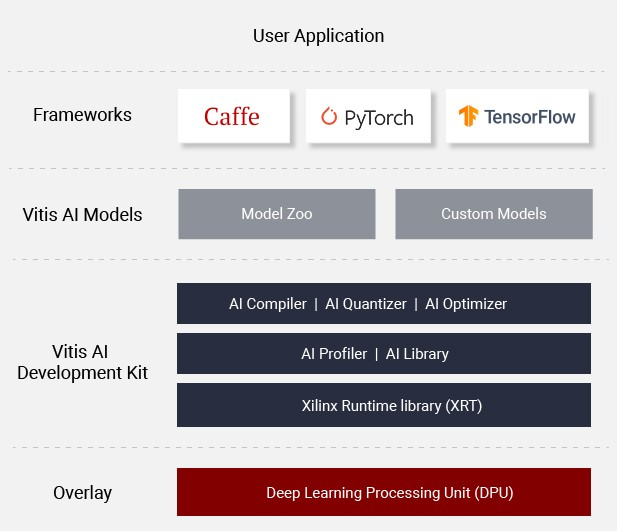
\includegraphics[width=\textwidth]{img/vitis-AI.jpg}
    \caption{Struktura narzędzia Vitis-AI}
    \label{vitisAI}
  \end{figure}

\subsection{Implementacja Sztucznych Sieci Neuronowych w układach FPGA}

Algorytmy wykorzystujące Sztuczne Sieci Neuronowe są dziś wykorzystywane w wielu zastosowaniach. Rozwój dziedziny Deep 
Learning spowodował powstanie modeli sieci zawierających wiele parametrów. Co za tym idzie, wzrosło zapotrzebowanie na metody 
akceleracji obliczeń w Sztucznych Sieciach Neuronowych. Większość obliczeń w ramach danej warstwy można zrównoleglić, więc 
zastosowania układów FPGA daje duże możliwości optymalizacji.

Najczęściej spotykanym podejściem jest zastosowanie ANN do wnioskowania (ang. \emph{inference}) nauczonej 
wcześniej sieci na nowych danych w czasie rzeczywistym. Model jest uczony na komputerze PC przy użyciu bibliotek takich jak 
\emph{keras}, \emph{Caffe} czy \emph{PyTorch}, najczęściej z wykorzystaniem GPU. Po przeprowadzeniu walidacji model sieci jest eksportowany, odpowiednio przetwarzany i implementowany w układzie FPGA. 


%przykłady implementacji

\subsubsection{Uczenie Sztucznej Sieci Neuronowej w układach FPGA}

Istnieje również możliwość zaimplementowania algorytmu uczenia ANN na układzie FPGA. Takie rozwiązanie pozwala na zrównoleglenie obliczeń, które jest istotne w przypadku wielu epok uczenia sieci, jednak wiąże się z następującymi problemami:
\begin{itemize}
    \item algorytm uczenia wymaga dużych zasobów pamięci
    \item skomplikowana implementacja algorytmu utrudnia wprowadzanie zmian w architekturze sieci
    \item implementacja modelu ze zmiennymi parametrami utrudnia optymalizację w HLS
\end{itemize}



% W tej pracy zastosowano architekturę sieci służącą do klasyfikacji obrazów odręcznie pisanych cyfr 